\section{Dissecting Modern Web Applications}
\paragraph{Architecture overview for web applications}
In order to properly understand how to apply the ideas of moving
target defense to web applications, we first describe a typical web application followed by a discussion on the ideas behind using moving target defense.
\begin{figure*}[tb]
	\centering
	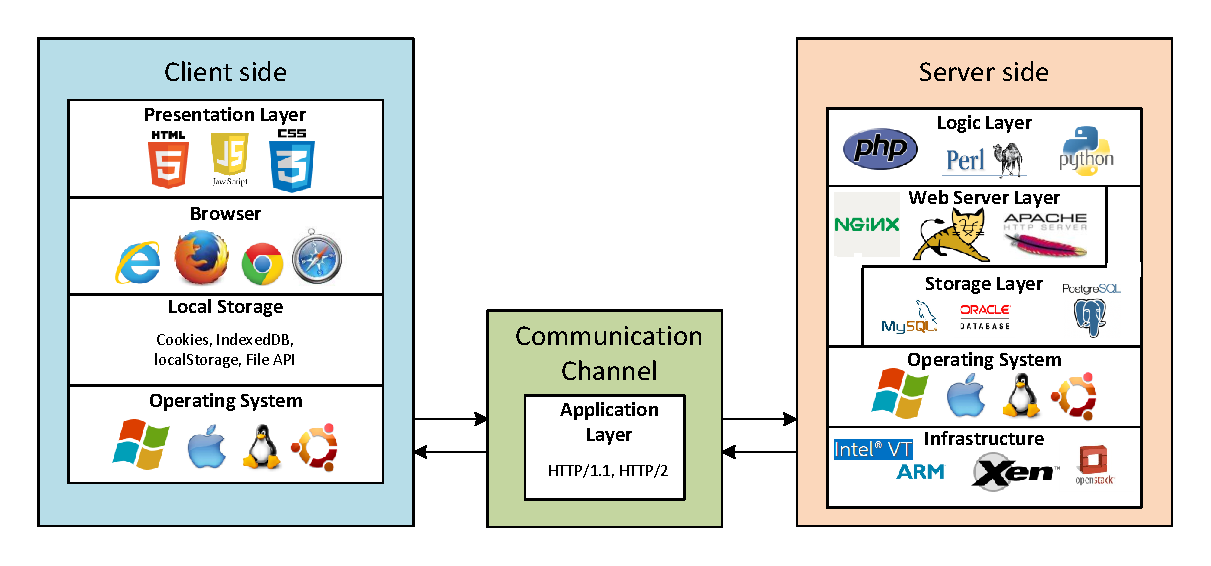
\includegraphics[width=.95\linewidth]{Web_App_Architecture}
	\caption{A Modern Web Application Architecture and Its Running Environments.}
	\label{fig:webapparch}
\end{figure*}
As shown in Figure~\ref{fig:webapparch}, a web application follows a
distributed application structure, with components running on both
server and the client systems.
\paragraph{Web application workflow and background}
When requesting a web resource, the client first issues a request to the server-side component over its communication channels - this is typically the HTTP protocol and its derivative protocols such as HTTPS, SPDY, and HTTP/2.
The server receives the request and processes it using the application's logic and returns the requested resource. If data stored in an external database is requested, the server passes the relevant user-input as a query and processes the result.
The server side typically includes the following layers from top to bottom\footnote{Of course, modern web application stacks can become increasingly complex, with caches, external requests, or other services, however we restrict our discussion to this abstracted model.}:
\begin{itemize}
	\item The server-side logic layer implements the application business logic using high-level programming languages, such as Java, PHP, or Python.
	\item The web server layer receives the HTTP request from the client, parses the HTTP request, and passes the request to the appropriate server-side program. Examples include Apache web server, Windows IIS, or Nginx.
	\item The data storage layer stores the web application state and user data. Popular data storage systems are traditional SQL databases, which include MySQL, PostgreSQL, or MSSQL.
	\item The operating system layer that provides the running environment for the web server layer and database storage layer.
	\item The infrastructure layer that runs the operating systems. An infrastructure could be a physical machine or a virtualization platform which manages multiple virtual machines.
\end{itemize}
The client receives the HTTP response from the server-side component and converts the HTML contained in the HTTP response into a graphical interface for the user.
The client consists of the following components:
\begin{itemize}
	\item The client-side logic layer, usually known as the presentation layer. The logic code here is usually composed of a combination of HTML, CSS, and JavaScript, with JavaScript providing a way for the server-side code to execute application logic on the client.
	\item The browser, which retrieves the presentation layer code from the server (typically HTML), interprets it, and presents it as a graphical interface to the user.
	\item The storage layer, that the presentation layer code uses to store data. Available storage methods include \verb"cookies", \verb"localStorage", \verb"IndexedDB", and File APIs.
	\item The operating system layer, which the browser runs on.
\end{itemize}